\chapter{基于深度相机模型形变捕捉}
要构建模型的形变子空间,除了静态三维模型,
还需要一些形变后的模型,即形变关键帧作为输入。
本章描述了一个以静态模型和深度视频为输入的形变捕捉算法。
在捕捉步骤中,操作者会带着特定颜色的手套,在深度相机前摆弄物体,使得物体发生形变。
该算法会优化模型的形变参数,使得模型的形状和相机采集的物体形状尽量吻合,
从而得到形变后的模型。
本文会从捕捉到的形变中选取若干成为形变关键帧,作为形变子空间构建的输入。
本章接下来就会阐述该算法的技术细节。

\section{基于手部信息的模型初始位姿确定}

 类似于三维重建步骤中的相机位姿估计,
 在形变步骤中,对于每一帧深度图像,本文仅计算模型和上一帧的相对形变。
 因此,在捕捉形变之前,需要得知模型的初始位置。
 由于在本文的形变捕捉流程中,需要用手持物体,所以

\subsection{基于颜色的手部点云分割}
\begin{figure}[h]
    \centering
    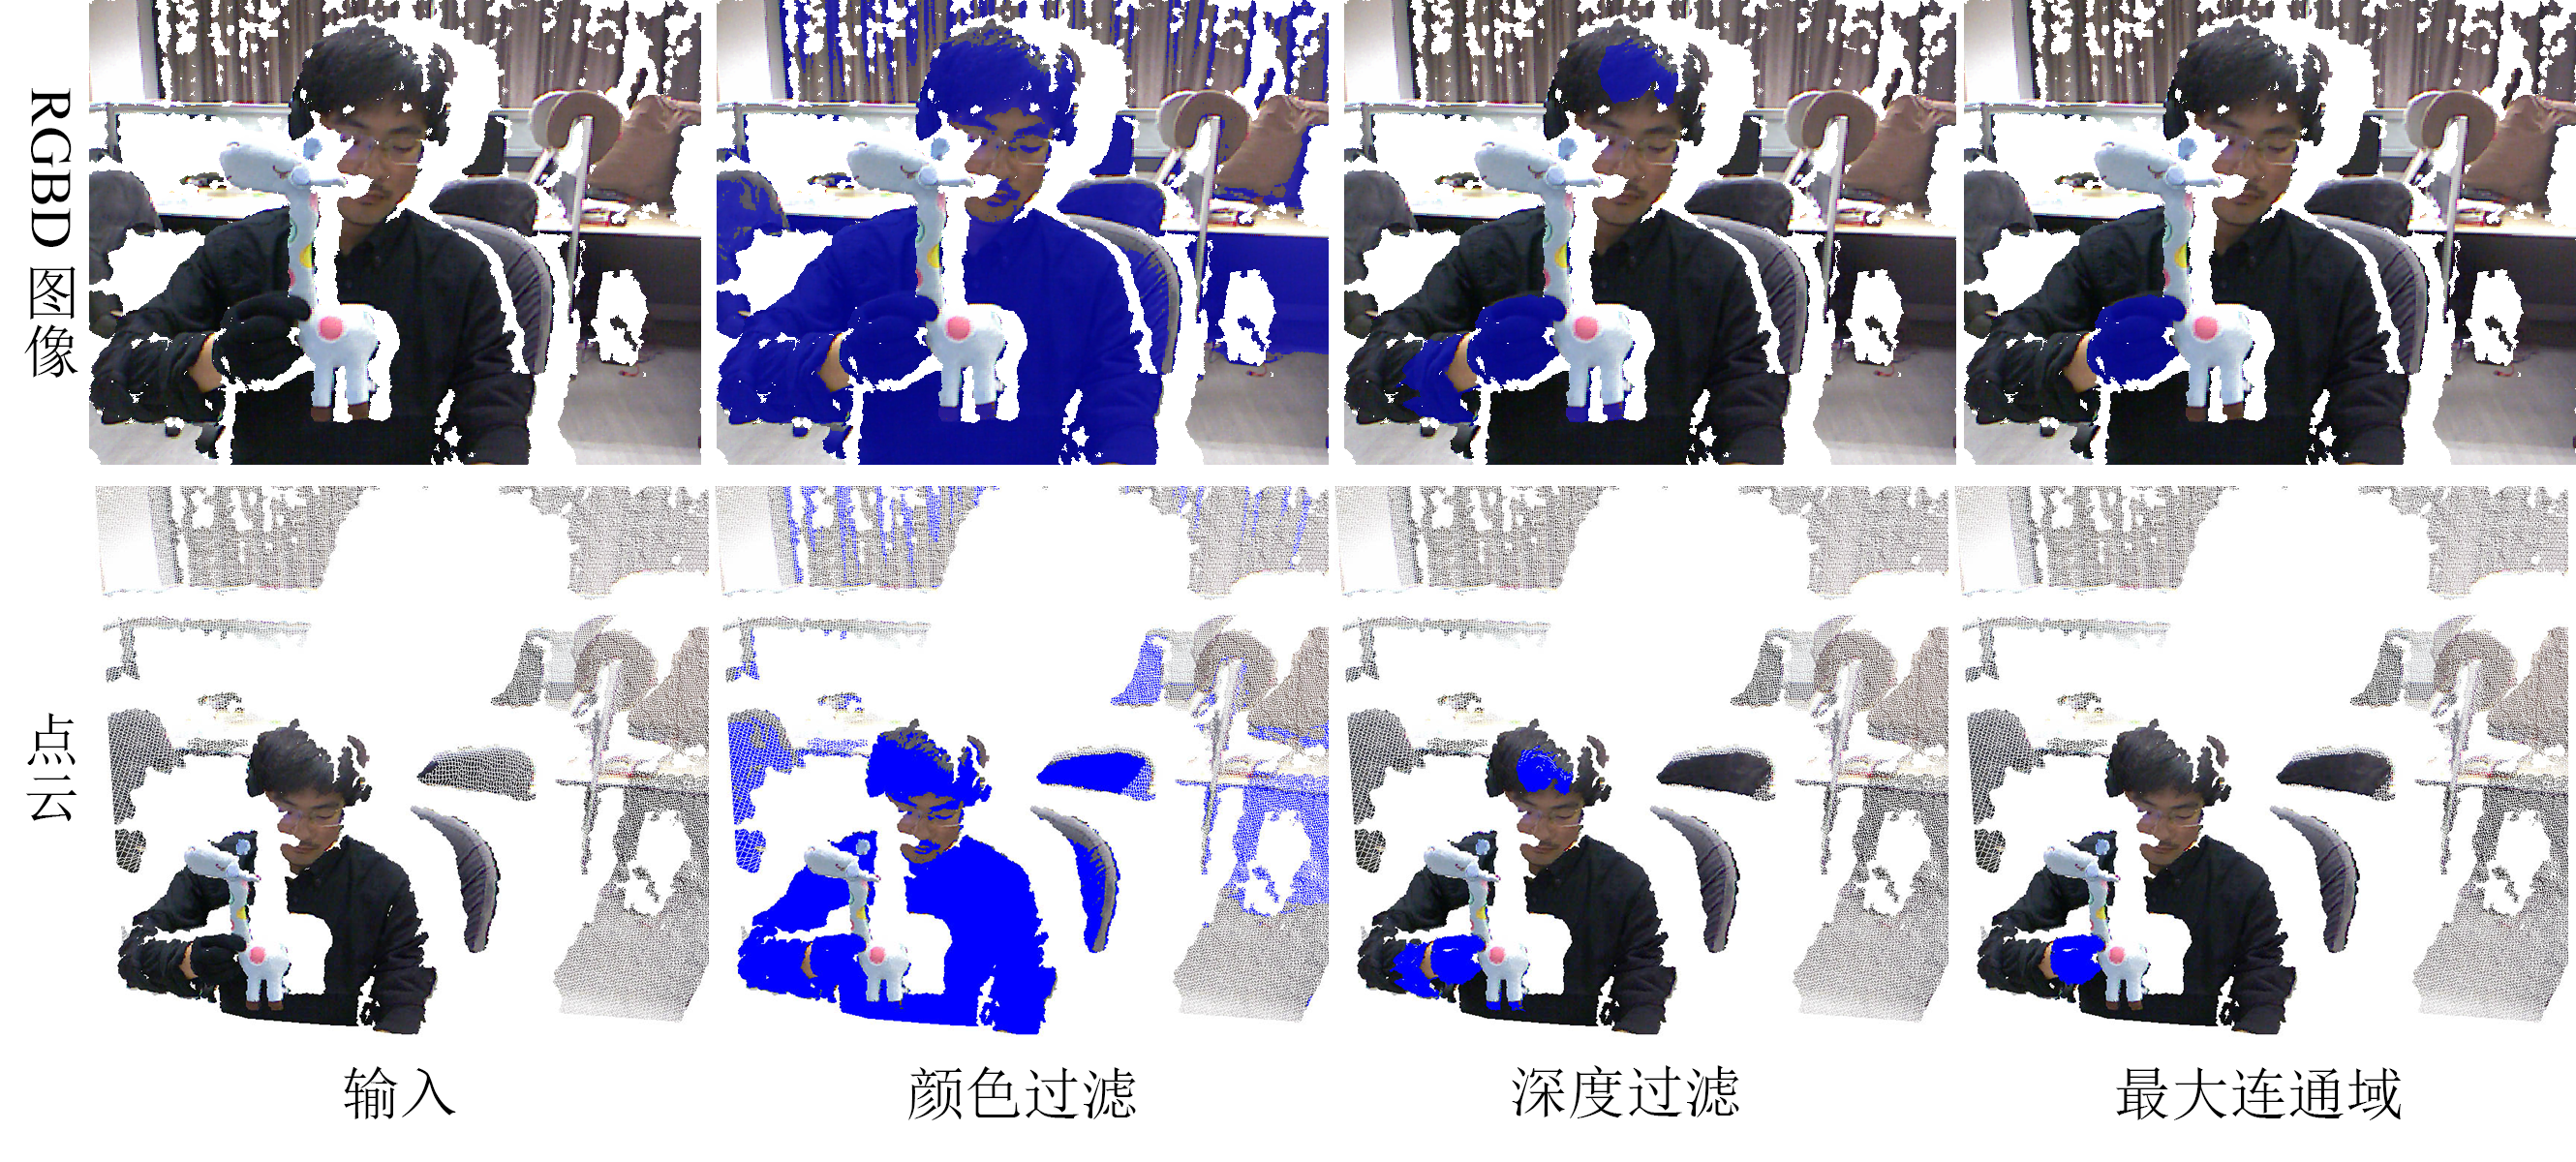
\includegraphics[width = \textwidth]{./Pictures/FindingHand.png}
    \caption{手部点云分割流程}
    \label{finding_hand}
\end{figure}
\subsection{基于手部位置的物体点云分割}
\subsection{模型对齐}

\section{基于深度视频的形变捕捉}
\subsection{形变的参数化描述}
\subsection{形变参数优化}

\section{本章小结}